\documentclass[tikz, border=3pt]{standalone}

\usepackage{tikz}
\usepackage{pgfplots}

\begin{document}
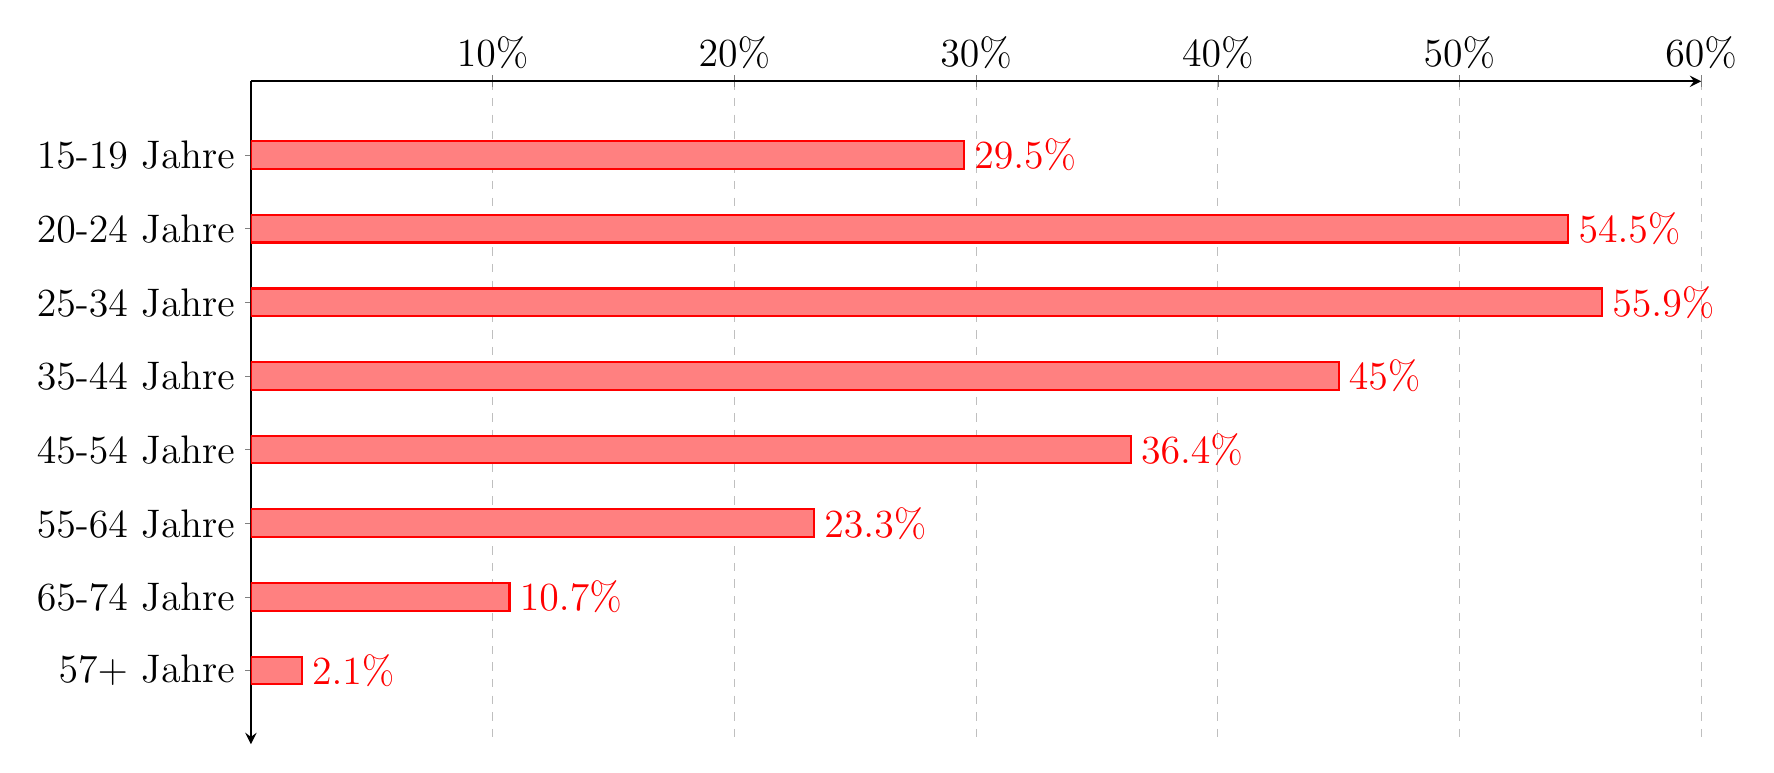
\begin{tikzpicture}

\begin{axis}[
	thick,
	xbar,
	xmin=0, xmax=60,
	ymin=0, ymax=9,
	width=20cm,
	height=10cm,
	xtick={10,20,30,40,50,60},
    ytick = {1,2,3,4,5,6,7,8},
	yticklabels={
		\Large 15-19 Jahre,
		\Large 20-24 Jahre,
		\Large 25-34 Jahre,
		\Large 35-44 Jahre,
		\Large 45-54 Jahre,
		\Large 55-64 Jahre,
		\Large 65-74 Jahre,
		\Large 57+ Jahre		
	},
	y dir=reverse,
	x tick label style={yshift=1mm,anchor=south},
	xticklabel={\Large\pgfmathprintnumber\tick\%},
	axis lines=middle,
    xmajorgrids,
    grid style={dashed},
    every axis x label/.style={
        at={(ticklabel* cs:0)},
        anchor=south west,
	},
]


	
% Cannabis
\addplot[ 
	color=red,
	fill=red!50!,
	bar width=10pt,
	nodes near coords=\Large\pgfmathprintnumber{\pgfplotspointmeta}\%,
] coordinates {
	(29.5, 1)
	(54.5, 2)
	(55.9, 3)
	(45.0, 4)
	(36.4, 5)
	(23.3, 6)
	(10.7, 7)
	(2.1, 8)
};


\end{axis}

\end{tikzpicture}
\end{document}